%%This is a very basic article template.
%%There is just one section and two subsections.
\documentclass[12pt,a4paper]{article}
\usepackage{ucs}
\usepackage[T2A]{fontenc}
\usepackage[utf8]{inputenc}
\usepackage[english,bulgarian]{babel}
\usepackage[margin=1in]{geometry}
\usepackage{listings}
\usepackage{color}
\usepackage{textcomp}
\usepackage[framed]{mcode}
\usepackage{graphicx}
\usepackage{caption}
\usepackage{subcaption}
\usepackage{amsmath}
\usepackage{setspace}

\addto\captionsbulgarian{%
  \renewcommand{\contentsname}%
    {Содржина}%
  \renewcommand{\tablename}%
    {Табела}%
  \renewcommand{\figurename}%
    {Слика}%
  \renewcommand{\bibname}%
    {Библиографија}%
  \renewcommand{\listfigurename}%
    {Листа на слики}%
  \renewcommand{\listtablename}%
    {Листа на табели}%
}
\renewcommand\lstlistingname{Код фрагмент}
\onehalfspacing
%\singlespacing

\begin{document}

\thispagestyle{empty}
\begin{titlepage}
\begin{center}
\newcommand{\HRule}{\rule{\linewidth}{0.5mm}}

% Upper part of the page

\includegraphics[width=0.15\textwidth]{images/ukim}\\[1cm]
\textsc{\large Универзитет „Св. Кирил и Методиј“ - Скопје}\\[1.5cm]


\includegraphics[width=0.3\textwidth]{images/finki_logo}\\[1cm]
\textsc{\large Факултет за информатички науки и компјутерско
инженерство}\\[1.5cm]

% Title
\HRule \\[0.4cm]
{  \bfseries \textsc{Имплементација на алгоритми од машинско учење во
Matlab/Octave} \\[0.4cm] - семинарска работа -}
\\[0.4cm]

\HRule \\[1.5cm]

% Author and supervisor
\begin{flushleft} 
\emph{Студиска програма:}\\
Компјутерски науки и инженерство\\
\emph{Предмет:}\\
MATLAB со примена на инженерски анализи\\
\emph{Студент:}\\
М-р Томче \textsc{Делев}\\
tomche.delev@finki.ukim.mk
\end{flushleft}

\vfill

% Bottom of the page
{\large Септември 2012}

\end{center}
\end{titlepage}

\tableofcontents
\newpage

\listoffigures

\newpage

\section{Вовед}

Машинско учење е подобласт на вештачката интелигенција. Со помош на алгоритми
таа се обидува да извлече што е можно повеќе корист од компјутерите кои
претставуваат најмоќни пресметковни машини. Примери на машинско учење се
рударењете на податоци од огромни бази на податоци, медицински записи, биолошки
податочни множества, како и ефикасното пребарување на веб. Голема примена наоѓа
и во области како обработка на природни јазици, препознавање на ракопис,
компјутерска визија итн.

Алгоритмите за машинско учење се подделени во две категории:
\begin{itemize}
  \item надгледувано учење,
  \item ненадгледувано учење.
\end{itemize}
Други видови на машинско учење вклучуваат засилено учење и системи за
препорачување.

Според резултатот од алгоритмот за машинско учење разликуваме алгоритми за
регресија и алгоритми за класификација. Во алгоритмите за регресија се
предвидува континуална променлива, додека во алгоритмите за класификација се
одредува класата (дискретна вредност) на примерокот кој се класифицира.


\section{Линеарна регресија}

\subsection{Линеарна регресија со една променлива}
Ова е имплементација на алгоритам за линеарна регресија кој го предвидува
профитот на камион кој превезува храна. Да предпоставиме дека вие сте извршен
директор на ланец ресторани и сакате да го проширите вашиот ланец во некој
друг град. Во ланецот веќе имате камиони во многу различни градови и имате
податоци за профитот и популацијата во тие градови. 

Сакате со помош на овие податоци да добиете помош кој да биде следниот ваш град
во кој ќе се проширите.

Во датотеката population\_profit.txt се наоѓа податочното множество за проблемот
на линеарна регресија. Во првата колона е популацијата на градот, а во втората е
профитот на камионот во тој град. Негативна вредност на профитот значи загуба.

\subsubsection{Исцртување на податоците}

Пред да се започне со било која обработка, вообичаено е корисно да се разберат
податоците со помош на визуелизација. За да ги визуелизираме овие податоци
користиме scatter plot, поради тоа што има само две својства кои се прикажуваат
(профит и популација).


\lstinputlisting[firstline=6,lastline=8,caption=Вчитување на податоците во променливите $X$ и $y$.
]{src/linearRegression/linearRegression.m}


\lstinputlisting[firstline=6,lastline=10,caption=Исцртување на податоците]{src/linearRegression/plotData.m}


\begin{figure}[htb]
\centering
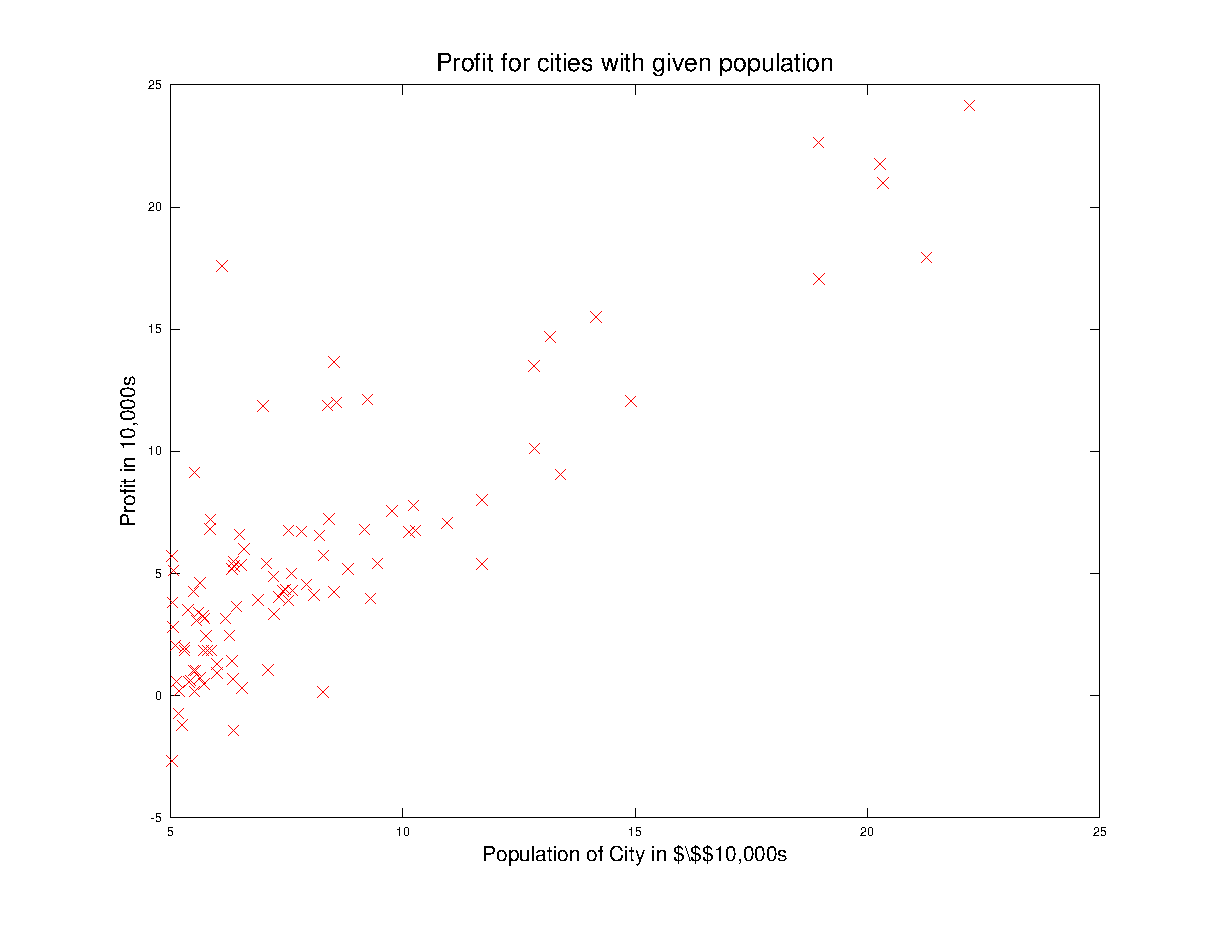
\includegraphics[width=.9\textwidth]{src/linearRegression/data}
\caption{Scatter plot на податочното множество}
\label{fig:plot}
\end{figure}

\subsubsection{Пресметување со Gradient Descent}

Следува имплементација на одредување на параметарот $\theta$ од лиенарната
регресија на податочното множество со помош на gradient descent.

\subsubsection{Равенки за пресметување}

Целта на линеарната регресија е да ја минимизира функцијата на чинење

\[
	J(\theta) = \frac{1}{2m}\sum^m_{i=1}{(h_\theta(x^{(i)}) - y^{(i)})^2}
\]
каде што хипотезата $h_\theta(x)$ е дадена со линеарниот модел:
\[
	h_\theta(x) = \theta^Tx = \theta_0 + \theta_1x_1
\]

Параметрите на моделот се вредностите $\theta_j$.
Алгоритмот го имплементираме со тоа што во секоја итерација ја извршуваме
следата формула:
\[
	\theta_j := \theta_j - \alpha\frac{1}{m}\sum^m_{i=1}{(h_\theta(x^{(i)}) -
	y^{(i)}) x_j}
\]
\emph{Симултано ги менуваме вредностите на $\theta_j$ за секое $j$.}

\subsubsection{Имплементација}

\lstinputlisting[firstline=23,lastline=28,caption=Додавање на дополнителна
колона $\theta_0$ и иницијализција на параметрите.]{src/linearRegression/linearRegression.m}

\subsubsection{Пресметување на функцијата на чинење $J(\theta)$}

\lstinputlisting[firstline=6,lastline=12,caption=Имплементација на
$J(\theta)$]{src/linearRegression/computeCost.m}

\subsubsection{Gradient Descent}

\lstinputlisting[firstline=6,lastline=16,caption=Имплементација
на Gradient Descent]{src/linearRegression/gradientDescent.m}

\begin{figure}[htb]
\centering
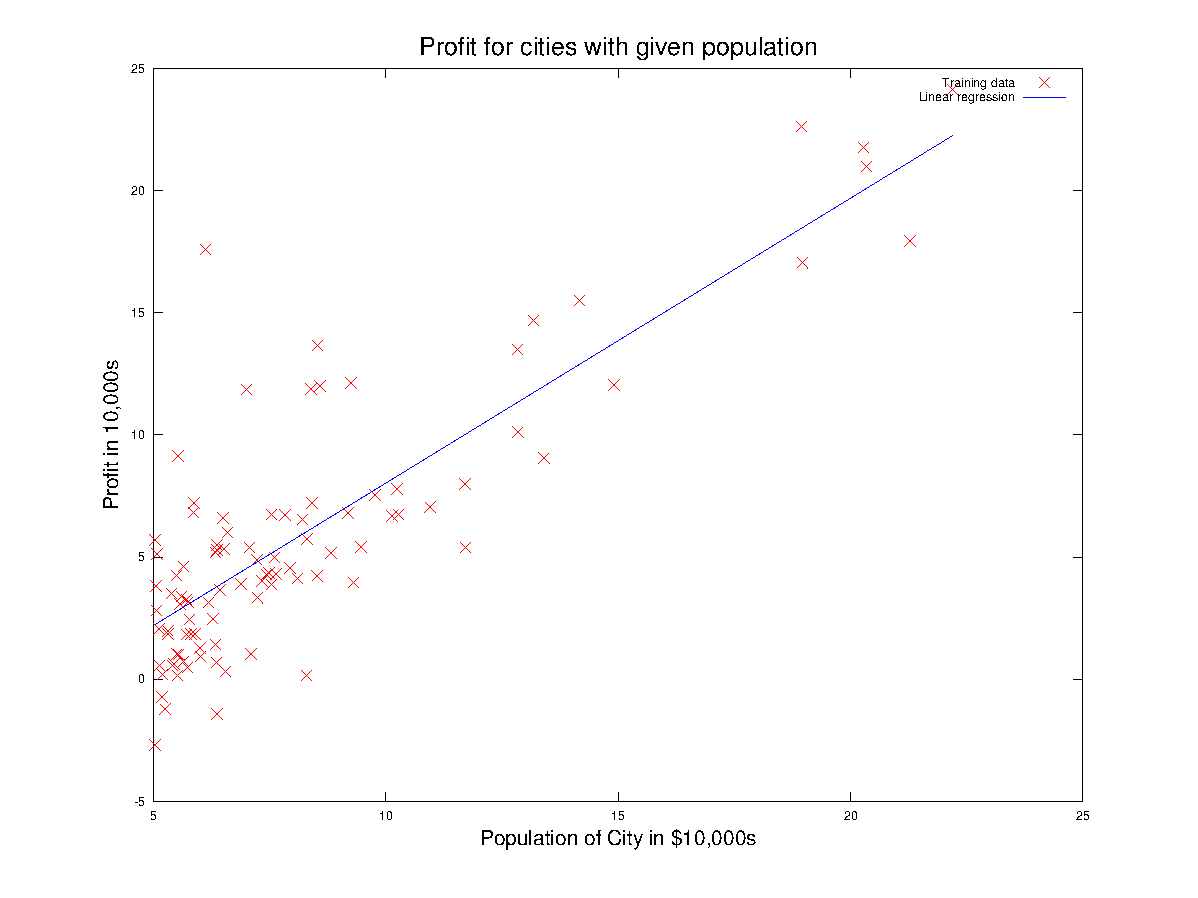
\includegraphics[width=.9\textwidth]{src/linearRegression/line_fit}
\caption{Линеарна регресија на тренинг множеството}
\label{fig:linear_fit}
\end{figure}

\subsubsection{Визуелизација на $J(\theta)$}
За подобро согледување на вредностите на функцијата на чинење $J(\theta)$ ги
исцртуваме нејзините вредност на 2-димензионален грид од вредностите
на $\theta_0$ и $\theta_1$.

Целта на овие графици е да покажат како $J(\theta)$ се менува со менувањето на
$\theta_0$ и $\theta_1$. Функцијата на чинење $J(\theta)$ е обликувана како
вдлабнат сад и има глобален минимум. Ова најубаво се воочува на површинскиот
график во 3Д. Минимумот е оптималната точка за $\theta_0$ и $\theta_1$, со што
алгоритмот gradient descent во секој чекор се доближува поблиску до оваа точка.


\begin{figure}[htbp]
        \begin{subfigure}[b]{0.5\textwidth}
                \centering
                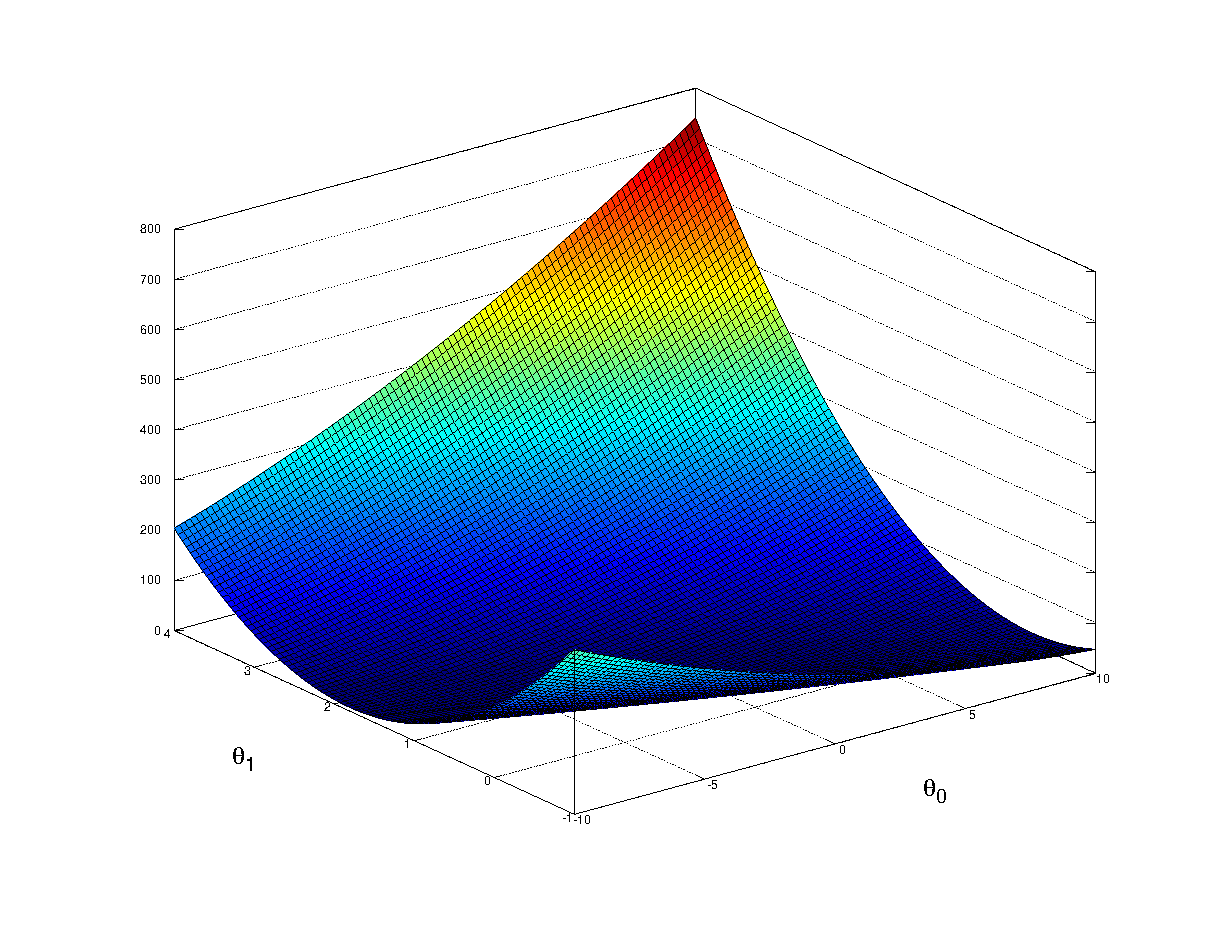
\includegraphics[width=\textwidth]{src/linearRegression/surface_plot}
                \caption{Површина}
                \label{fig:surface}
        \end{subfigure}%
        ~ 
        \begin{subfigure}[b]{0.5\textwidth}
                \centering
                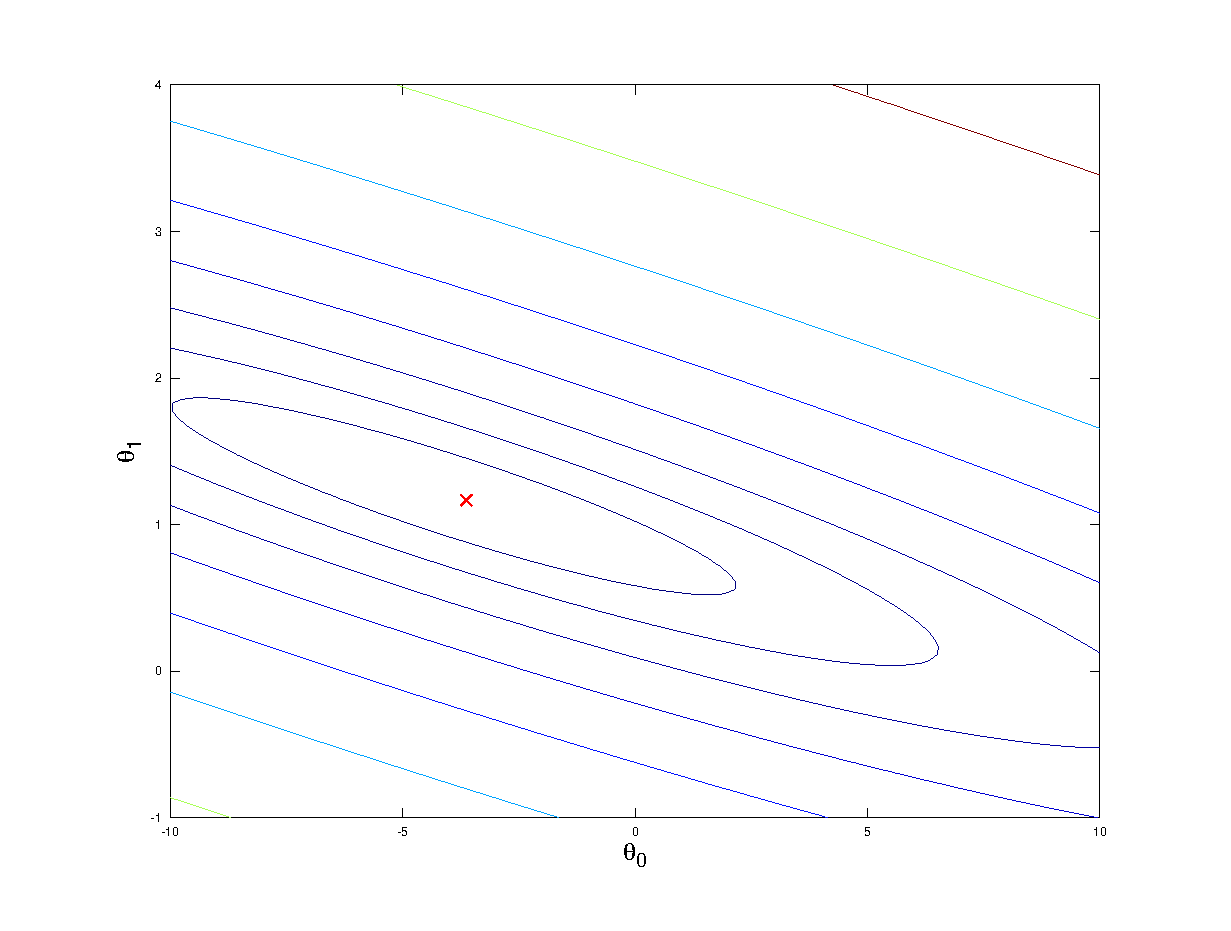
\includegraphics[width=\textwidth]{src/linearRegression/contour}
                \caption{Контура која го прикажува минимумот}
                \label{fig:contour}
        \end{subfigure}
        \caption{Функцијата на чинење $J(\theta)$}
        \label{fig:cost_function}
\end{figure}

\subsection{Линеарна регресија со повеќе променливи}

Со помош на линеарна регресија со повеќе променливи ќе ја предвидуваме цената на
куќите. Да претпоставиме дека продаваме куќа и сакаме да дознаеме која е
нејзината цена на пазарот. Еден начин да го дознаеме ова е да собереме
информации за цените на последно продадените куќи ид да изградиме модел на
цените на куќите.

Во датотеката houses\_prices.txt се содржи податочно множество со цените на
куќите во Портланд, Орегон. Првата колона е големината на куќата (во квадратни
стапки), втората колона е бројот на соби, а третата колона е цената на куќата.

\subsubsection{Нормализација на обележјата}

Помеѓу вредностите на некои обележја постојат многу големи разлики и тоа не е
добро за алгоритмите за машинско учење. Затоа кога постојат вакви огромни
разлики, вредностите на обележјата се нормализираат (скалираат) со што
алгоритмот gradient descent многу побрзо конвергира. 

Нормализацијата ја извршуваме со следните чекори:
\begin{itemize}
  \item Ја одземаме средната вредност од секое обележје во податочното
  множество,
  \item Ги скалираме (делиме) вредностите на обележјата со нивните соодветни
  стандардни девијации.
\end{itemize}

\lstinputlisting[firstline=8,lastline=16,caption=Нормализација
на обележјата]{src/linearRegression/featureNormalize.m}


\subsubsection{Gradient Descent}

\lstinputlisting[firstline=6,lastline=18,caption=Имплементација
на Gradient Descent за повеќе
променливи]{src/linearRegression/gradientDescentMulti.m}


\subsubsection{Нормални равенки}
Точното решение на линеарна регресија може да се определи со равенката:

\[
	\theta = (X^TX)^{-1}X^T\vec{y}.
\]

За да се употребува оваа формула не е потребно скалирање на обележјата и ќе се
добие точно решение во една пресметка: нема „циклус до конвергенција“ како во
претходниот алгоритам.



\section{Логистичка регресија}

Со овој алгоритам ќе изградиме модел за логистичка регресија кој ќе предвидува
дали кандидатот е примен или не на универзитет.

Вие сте раководител на некој оддел во универзитет и сакате да ги одредите
шансите на кандидатот да биде примен во зависност од неговите резултати на двата
приемни испити. Поседувате податоци од претходните уписи со резултатите од двата
испити и одлуката дали е примен кандидатот или не.

Целта е да се изгради модел за класификација кој ќе ја предвидува веројатноста
за да биде примен кандидатот во зависност од резултатите од двата испити.

\subsection{Визуелизација на податоците}
На слика \ref{fig:plot2} е прикажана визуелизација на податоците од податочното
множество, во кое со жолти кругчиња се означени одбиените, а со црвени плус
знаци примените кандидати.

\begin{figure}[htb]
\centering
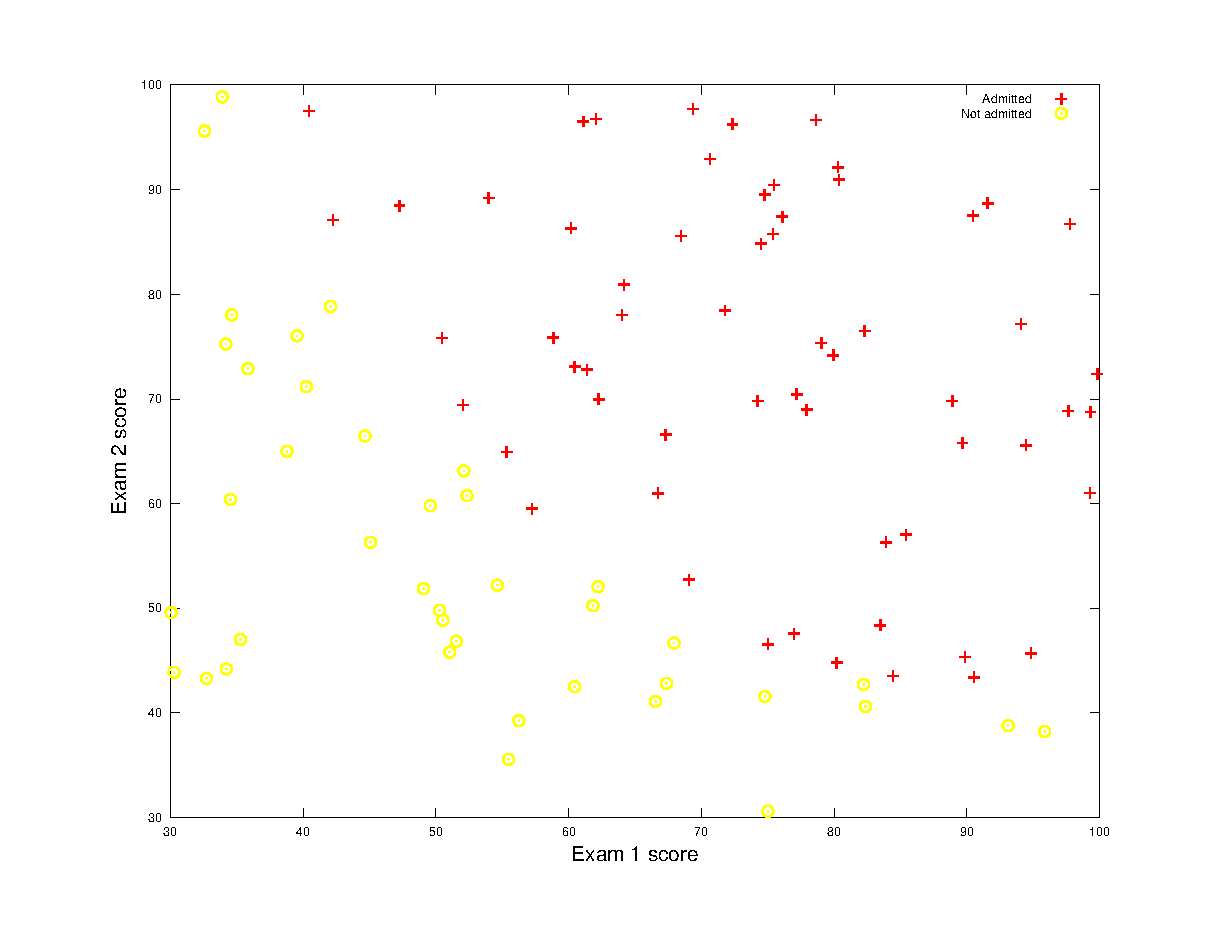
\includegraphics[width=.9\textwidth]{src/logisticRegression/data}
\caption{Scatter plot на податочното множество}
\label{fig:plot2}
\end{figure}

\lstinputlisting[firstline=9,lastline=16,caption=Разделување на податочното
множество на позитивни и негативни примероци и негова визуелизација]{src/logisticRegression/plotData.m}

\subsection{Имплементација}

\subsubsection{Sigmoid функција}

Хипотезата во логистичка регресија е дефинирана со:

\[
	h_{\theta}(x) = g(\theta^Tx),
\]
каде функцијата $g$ e sigmoid функцијата. Sigmoid функцијата е дефинирана со:

\[
	g(z) = \frac{1}{1 + e^{-z}}
\]

\lstinputlisting[firstline=5,lastline=6,caption=Имплементација
на функцијата sigmoid]{src/logisticRegression/sigmoid.m}

Функцијата на чинење во логистичка регресија е:

\subsubsection{Функција на чинење и градиент}
\[
	J(\theta) = \frac{1}{m}\sum^m_{i=1} \left[ -y^{(i)} \log(h_\theta(x^{(i)})) -
	(1 - y^{(i)})\log(1 - h_\theta(x^{(i)})) \right]
\]

а градиентот на чинење е вектор со иста должина како $\theta$ каде што $j^{th}$
елемент (за $j = 0, 1, \ldots ,n$) е дефиниран на следниот начин:
\[
	\frac{\partial J(\theta)}{\partial\theta_j} =
	\frac{1}{m}\sum^m_{i=1}{(h_\theta(x^{(i)}) - y^{(i)})}x^{(i)}_j
\]

\subsubsection{Учење на параметрите со \texttt{fminunc}}
Учењето на параметрите $\theta$ во овој алгоритам ќе го правиме со употреба со
готовата функција за минимизација \texttt{fminunc}. Ова е вградена функција која
наоѓа минимум на неограничена \footnote{Ограничувањата во оптимизацијата често се однесуваат на ограничувања на
параметрите, на пример, ограничувања на вредностите на $\theta$ (пр., $\theta
<= 1$). Логистичката регресија нема такви ограничувања затоа што $\theta$ може
да ја прими вредноста на секој реален број.} функција.

За логистичка регресија ја оптимизираме функцијата на чинење $J(\theta)$ со
параметар $\theta$.

Конкретно, ќе ја користиме fminunc да ги пронајдеме најдобрите параметри
$\theta$ за функцијата на чинење на логистичката регресија, за дадено податочно
множество (X и y вредности). Функцијата fminunc ќе ја повикаме со следните
аргументи:
\begin{itemize}
  \item Иницијалните вредности на параметрите кои сакаме да ги оптимизираме.
  \item Функција, која за дадено тренинг податочно множество и дадено $\theta$,
  пресметува функција на чинење на логистичка регресија и градиент.
\end{itemize}

\lstinputlisting[firstline=50,lastline=58,caption=Повикување
на функцијата за оптимизација
\texttt{fminunc}]{src/logisticRegression/logisticRegression.m}

Со овој код фрагмент, најпрво ги дефинираме опциите со кои ќе ја повикаме
\texttt{fminunc}. Со поставување на \texttt{GradObj} на \texttt{on}, ѝ
кажувме на \texttt{fminunc} дека нашата функција враќа и чинење и градиент.
Ова овозможува \texttt{fminunc} да го користи градиентот за минимизирање на
функцијата. Со поставување на \texttt{MaxIter} на 400, ја ограничуваме
\texttt{fminunc} да се извршува максимум 400 итерации.

\begin{figure}[htb]
\centering
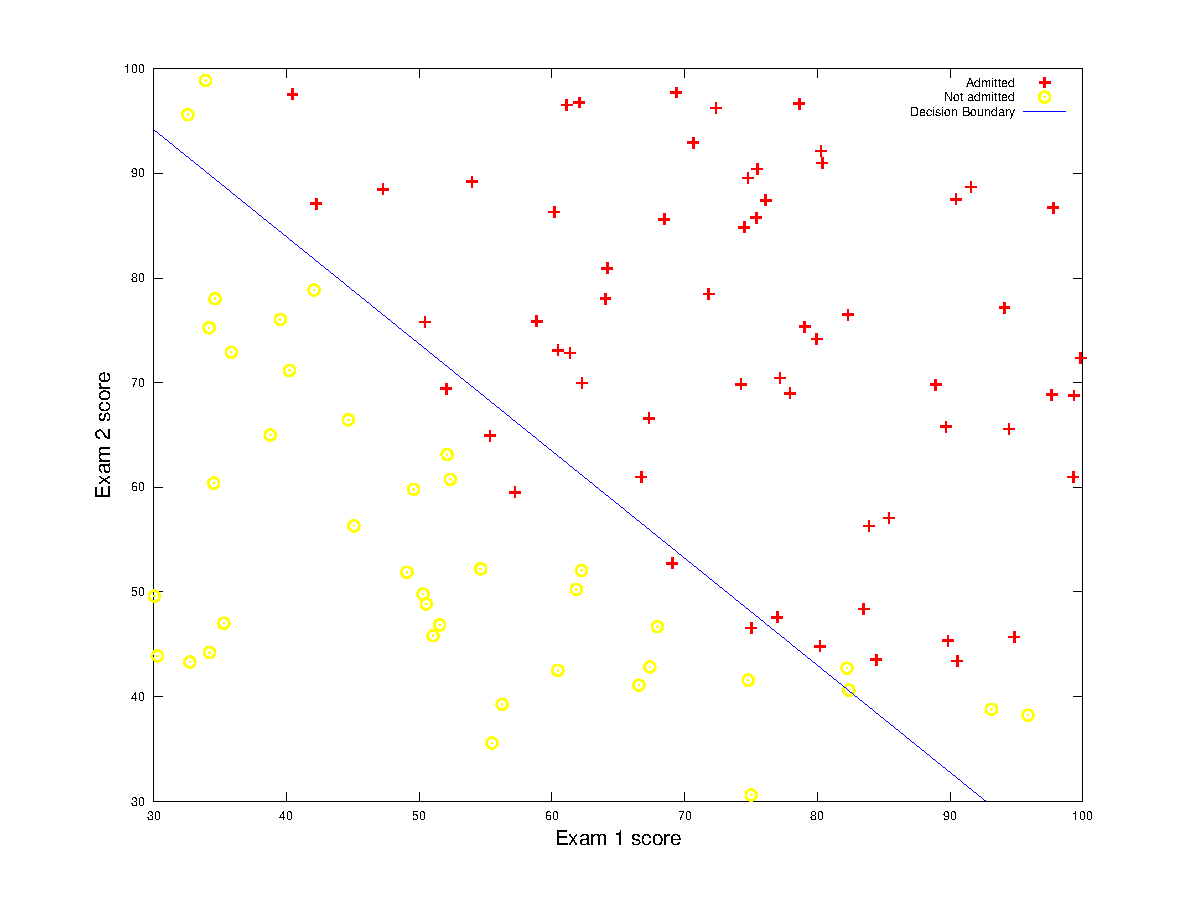
\includegraphics[width=.9\textwidth]{src/logisticRegression/decisionBoundary}
\caption{Податочното множество со границата на одлука}
\label{fig:decisionBoundary}
\end{figure}

Вредноста на $\theta$ која се добива како резултат на оптимизацијата служи за
исцртување на границата на одлука прикажана на слика \ref{fig:decisionBoundary}.

\subsubsection{Евалуација на логистичката регресија}

Откако ќе ги научиме параметрите, го користиме моделот за да предвидиме дали
одреден кандидат ќе биде примен. За кандидат кој на првиот испит имал 45 поени,
а на вториот 85, добиваме веројатност за успех од 0.776.

Нашиот модел го евалуираме на целото тренинг множество.

\lstinputlisting[firstline=7,lastline=10,caption=Функцијата
за евалуација на тренинг множеството]{src/logisticRegression/predict.m}


\section{Невронски мрежи}

Имплементација на алгоритмот за повратна пропагација за учење на параметрите на
невронската мрежа. Овој алгоритам ќе го искористиме за препознавање на ракописно
напишани цифри. Ова е корисно во автоматско читање на поштенски кодови, чекови,
сметки и слично.

\subsection{Визуелизација на податоците}

\begin{figure}[htb]
\centering
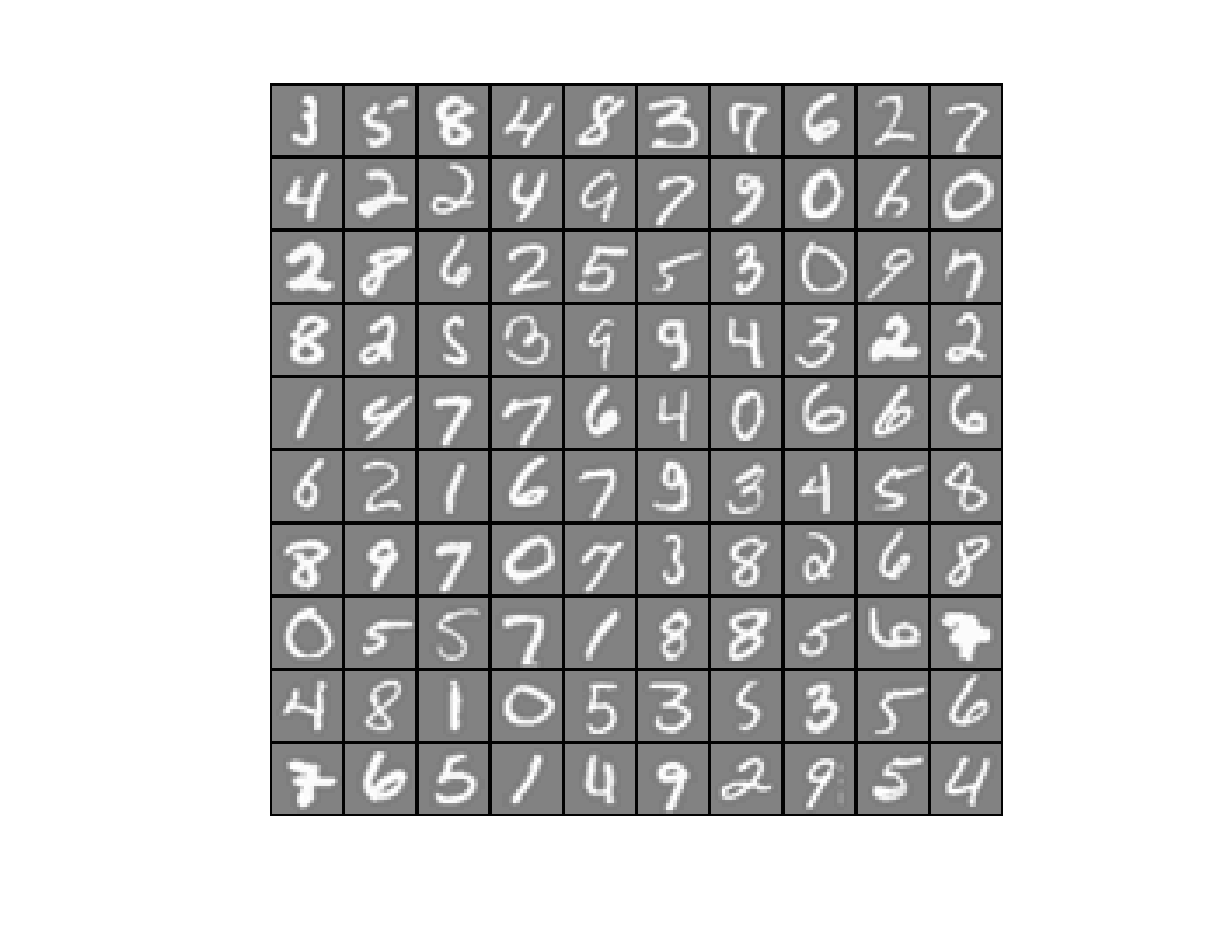
\includegraphics[width=.9\textwidth]{src/neuralNetwork2/nn}
\caption{Примероци од податочното множество}
\label{fig:neuralNetworkData}
\end{figure}

Податочното множество (дел е прикажан на слика \ref{fig:neuralNetworkData}) за овој алгоритам е
составено од 5000 тренинг примероци, од кој секој примерок е црно-бела слика од 20x20 пиксели. Секој пиксел се
репрезентира со децимален број кој го означува интензитетот. Овие 400 пиксели се
сместени во еднодимензионален вектор. Секој од овие тренинг примероци
претставува ред од матрицата X. Со ова се добива матрица од 5000 по 400 во која
секој ред е примерок за слика од ракописно напишана цифра.

\[
	X = \begin{bmatrix}
		    (x^{(1)})^T \\
			(x^{(2)})^T \\
			\vdots \\
			(x^{(m)})^T
			
		\end{bmatrix}
\]

Вториот дел од податочното множество е 5000-димензионален вектор $y$ кој 
ги содржи целните ознаки за податочното множество. За да се постигне
компатибилност со индексирањето во Octave/Matlab, каде што не постои 0 индекс,
цифрата 0 е пресликана во вредноста 10. Така, цифрата „0“ е означена како „10“,
додека цифрите од „1“ до „9“ се означени како „1“ до „9“ во нивниот природен
редослед.

\subsection{Репрезентација на моделот}

\begin{figure}[htb]
\centering
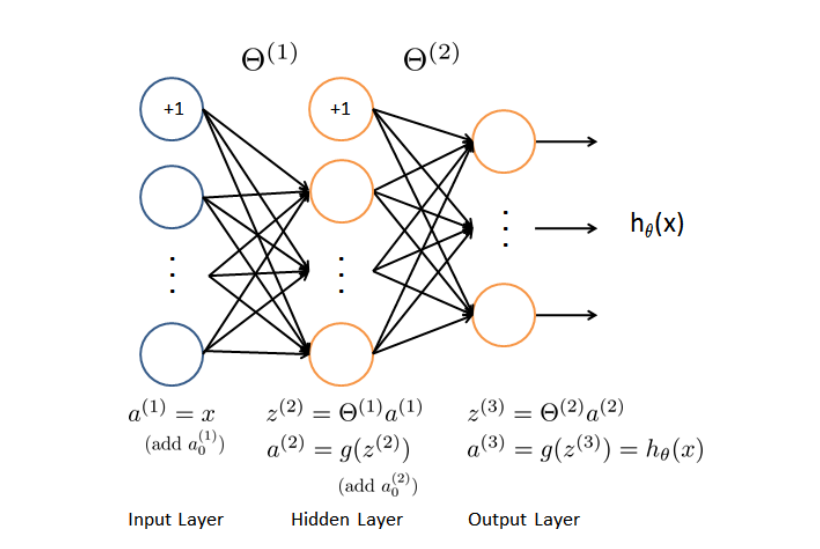
\includegraphics[width=.9\textwidth]{src/neuralNetwork2/neuralNetwork}
\caption{Моделот на невронска мрежа}
\label{fig:neuralNetwork}
\end{figure}

На слика \ref{fig:neuralNetwork} е прикажан моделот на невронската мрежа. Се
состои од 3 слоеви: влезен слој, скриен слој и излезен слој. На влезот на оваа
невронска мрежа се дигиталните слики. Затоа што секоја слика е со големина 20 x
20, влезниот слој е составен од 400 влезни единици.

\subsection{Feedforward пропагација и предикција}

Алгоритмот за feedforward пропагација ја пресметува $h_\theta(x^{(i)})$ за секој
примерок $i$ и ја враќа предвидената вредност. Слично како кај стратегијата за класификација
еден-против-сите, предвидувањето на невронската мрежа ќе биде ознаката со
најголема вредност $(h_\theta(x))_k$.

\lstinputlisting[firstline=6,lastline=17,caption=Имплементација
на функцијата predict]{src/neuralNetwork1/predict.m}


\subsection{Feedforward и cost функција}

Функцијата на чинење на невронска мрежа (без регуларизација) е

\[
	J(\theta) = \frac{1}{m}\sum_{i = 1}^{m}\sum_{k =
	1}^{K}[-y^{(i)}_k\log((h_\theta(x^{(i)}))_k) -
	(1 - y^{(i)}_k)\log(1 - (h_\theta(x^{(i)}))_k)],
\]

каде што $h_\theta(x^{(i)})$ се пресметува како на слика \ref{fig:neuralNetwork}
 и $K = 10$ е бројот на можни ознаки. Со $(h_\theta(x^{(i)}))_k = a^{(3)}_k$ се
 означува активацијата (излезната вредност) на $k-th$ излезна единица.
 Оригиналните вредности за излезната ознака $y$ се 1, 2, \ldots, 10, за
 тренирање на невронска мрежа, треба сите ознаки да се претворат во соодветни
 вектори кои ги содржат единствено вредностите 0 и 1:
 
 \[	
	y = \begin{bmatrix}
		    1 \\
			0 \\
			0 \\
			\vdots \\
			0
			
		\end{bmatrix},
		\begin{bmatrix}
		    0 \\
			1 \\
			0 \\
			\vdots \\
			0
			
		\end{bmatrix},
		\ldots
		or
		\begin{bmatrix}
		    0 \\
			0 \\
			0 \\
			\vdots \\
			1
			
		\end{bmatrix}
 \]

На пример, ако $x^{(i)}$ е слика од цифрата 5, тогаш соодветното $y^{(i)}$ (кое
треба да се искористи во функцијата на чинење) треба да биде 10-димензионален вектор
со $y_5 = 1$, а останатите елементи 0.

\lstinputlisting[firstline=17,lastline=60,caption=Имплементација
на функцијата на
чинење,basicstyle=\ttfamily\scriptsize]{src/neuralNetwork2/nnCostFunction.m}

\subsection{Backpropagation}

\subsubsection{Сигмоид градиент}

Градиентот за сигмоид функцијата се пресметува како

\[
	g'(z) = \frac{d}{dz}g(z) = g(z)(1 - g(z))
\]

каде што

\[
	sigmoid(z) = g(z) = \frac{1}{1 + e^{-z}}.
\]

\subsubsection{Случајна иницијализација}

Кога се тренираат невронски мрежи, важно е да параметрите да се иницијализираат
случајно за да се наруши симетријата. Една ефективна стратегија за случајна
иницијализација е случајно да се изберат вредности за $\theta(l)$ рамномерно во
опсегот $[-\epsilon_{init}, \epsilon_{init}]$. Овој опсег не осигурува дека
вредностите на параметрите ќе бидат мали, а со тоа и учењето ќе биде поефикасно.

\lstinputlisting[firstline=14,lastline=16,caption=Имплементација
на случајна иницијализација]{src/neuralNetwork2/randInitializeWeights.m}

\subsubsection{Backpropagation}

\begin{figure}[htb]
\centering
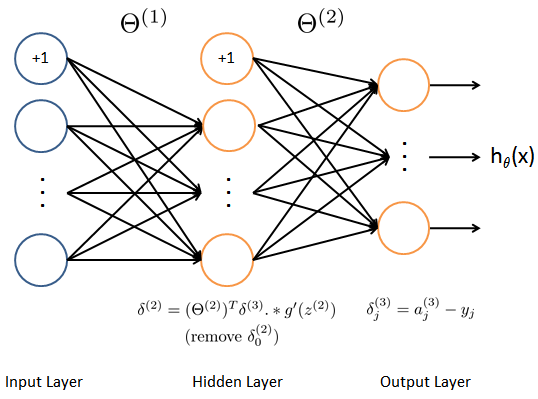
\includegraphics[width=.9\textwidth]{src/neuralNetwork2/nnb}
\caption{Освежување на вредностите во Backpropagation}
\label{fig:backpropagation}
\end{figure}

За даден тренинг примерок $(x^{(t)}, y^{(t)})$, најпрво се извршува „изминување
нанапред“ за да се добијат активациските вредности во мрежата, вклучувајќи ги и
излезните вредности на хипотезата $h_\theta(x)$. Потоа, за секој јазел $j$ во
слојот $l$, сакаме да ја пресметаме „грешката“ $\delta_j^{(l)}$ која означува
колку секој јазел во мрежата е „одговорен“ за грешките во излезот.

За излезните јазли, можеме директно да ја измериме разликата меѓу активацијата
на мрежата и вистинската вредност и да ја искористиме за да ја дефинираме
$\delta_j^{(3)}$ (слојот 3 е излезниот слој). а скриените единици,
$\delta_j^{(l)}$ го пресметуваме како тежински просек на изразите за грешка на
слојот $(l + 1)$.

Детално чекорите на backpropagation алгоритмот се следните:

\begin{enumerate}
  \item Поставете ги вредностите на влезниот слој $(a^{(1)})$ на вредностите од
  $t-$тиот тренинг примерок $x^{(t)}$. Следува feedforward (Слика
  \ref{fig:backpropagation}), за пресметување на активациите $z^{(2)}, a^{(2)},
  z^{(3)}, a^{(3)}$ за слоевите 2 и 3. Исто така треба да се додаде и изразот a + 1 за да активациските
  вектори за слоевите $a^{(1)}$ и $a^{(2)}$ исто така ја вклучуваат единицата
  за наклонетост. Во Matlab и Octave, ако 1 е вектор колона, додавање 1 е
  еквивалентно на \begin{verbatim} a_1 = [1; a_1]. \end{verbatim}
  \item За секоја излезна единица $k$ во слојот 3 (излезниот слој), пресметајте:
  \[
  	\delta_k^{(3)} = (a^{(k)} - y_k),
	\]
	каде што $y_k $ покажува дали тековниот примерок припаѓа на класата $k (y_k =
	1)$ или припаѓа на друга класа $(y_k = 0)$.
  \item За скриениот слој $l = 2$, пресметајте
   	\[
  	\delta^{(2)} = (\Theta^{(2)})^T \delta^{(3)} .* g'(z^{(2)}),
	\]
	\item Соберете го градиентот од овој примерок со користење на следната формула:
	\[
  	\Delta^{(l)} = \Delta^{(l)} + \delta^{(l + 1)}(a^{(l)})^T
	\]
	\item Пресметајте го (ненормализираниот) градиент за функцијата на чинење на
	неверонската мрежа со множење на збирот на градиентите со $\frac{1}{m}$:
	 \[
  	\frac{\partial}{\partial\Theta_{ij}^{(l)}} J(\Theta) = D_{ij}^{(l)} =
  	\frac{1}{m}\Delta_{ij}^{(l)}
	\]
	
\end{enumerate} 


\begin{figure}[htb]
\centering
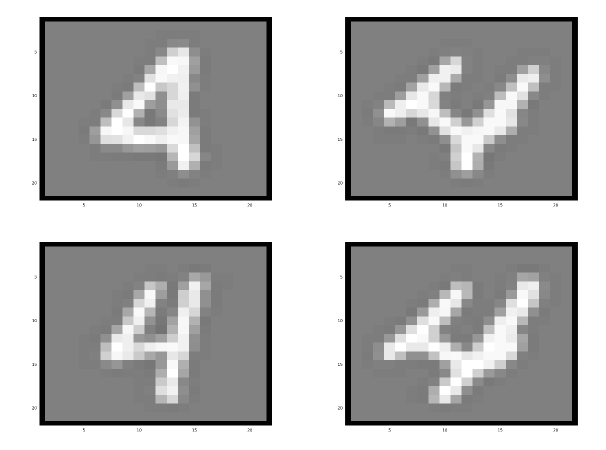
\includegraphics[width=.6\textwidth]{src/neuralNetwork1/num_4}
\caption{Четири различни прикази на бројот 4}
\label{fig:num4}
\end{figure}

\begin{figure}[htb]
\centering
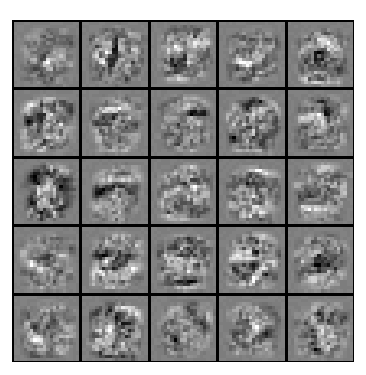
\includegraphics[width=.6\textwidth]{src/neuralNetwork2/nn_viz}
\caption{Визуелизација на тренираната невронска мрежа}
\label{fig:viz}
\end{figure}

\subsection{Примери}

На слика \ref{fig:num4} се прикажани четири различни примериоци на бројот 4 и во
сите случаи алгоритмот точно ја предвидува прикажаната бројка. На слика
\ref{fig:viz} е прикажана визуелизација на тренираната невронска мрежа.







\newpage

\nocite{*}
\bibliographystyle{amsplain}
\bibliography{ref}

\end{document}
